\documentclass[slidestop,compress,xcolor=dvipsnames]{beamer}
%\usetheme{Antibes}
%\usetheme{Boadilla}
%\usetheme{JuanLesPins}
\usetheme{Frankfurt}

%\xdefinecolor{rgb}{LemonChiffon}{0.98,0.98,0.8}
%\xdefinecolor{rgb}{LightBlue}{0.68,0.85,0.9}
%\newcommand{\mblue}{\blue}
%\newcommand{\mgreen}{\green}
%\newcommand{\mred}{\red}
%\xdefinecolor{rgb}{mgreen}{0,0.4,0.5}
%\xdefinecolor{rgb}{agreen}{0.2,0.5,0.1}
\xdefinecolor{lavender}{rgb}{0.8,0.6,1}

\newcommand{\colred}{\textcolor{red}}
\newcommand{\colblue}{\textcolor{blue}}
\newcommand{\colgreen}{\textcolor{green}}
%\newcommand{\colgreenb}{\textcolor{darkgreen}}
\newcommand{\colpurple}{\textcolor{purple}}

\newcommand{\methaddcol}{\colpurple}

\definecolor{shade}{gray}{0.9}

\newcommand{\lcaporali}{{\fontencoding{T1}\fontfamily{ptm}\selectfont<<}}
\newcommand{\rcaporali}{{\fontencoding{T1}\fontfamily{ptm}\selectfont>>}}

%\usepackage[bars]{beamerthemetree}
%\usepackage{beamerthemeshadow}
%\usepackage{mathpazo}
%\usepackage{listings}
\usepackage{graphicx}
\usepackage{color}
\usepackage{pgf}
\usepackage{mathpartir}
\usepackage{xspace}

\usepackage[latin1]{inputenc}
\usepackage[percent]{overpic}
\usepackage{tikz}
\let\Tiny=\tiny
\newcommand{\g}{\ensuremath{\Gamma}}
\newcommand{\f}{\ensuremath{\vdash}}
\newcommand{\T}{\mytt{T}}

\newcommand{\mytt}[1]{\textup{\texttt{#1}}}
\newcommand{\mykeyb}[1]{\textup{\textbf{#1}}}

\newcommand{\checkm}{\mytt{@Check}}

\newcommand{\failedexc}{\mytt{RuleFailedException}}
\newcommand{\ruleapptrace}{\mytt{RuleApplicationTrace}}

\usepackage{tabularx}  

\newcommand{\br}{\texorpdfstring{\\}{}}

\usepackage{pgfpages}
% use \notes{} to insert notes
% create pdf twice as wide with notes (needs package pgfpages)
%\setbeameroption{show notes on second screen}


\title{Type System Frameworks for Xtext}
\author{\textbf{Lorenzo Bettini}$^1$ \and \textbf{Dietmar Stoll}$^2$\\
joint work with\\
\textbf{Serano Colameo}$^2$ \and \textbf{Markus V\"olter}$^3$}
\institute{$^1$Dipartimento di Informatica, Universit\`a di Torino, Italy\\
$^2$Itemis GmbH, Zurich, Switzerland\\
$^3$Itemis AG, Stuttgart, Germany}
\date{Eclipse Day Florence, May 4th, 2012}

\begin{document}
\maketitle

\section*{Outline}
\begin{frame}
   \tableofcontents
\end{frame}

\section{Introduction}
\label{sec:introduction}

Developing a compiler for a language and its integration in Eclipse is usually
time consuming since it requires many phases, starting from parsing the program,
checking that is correct, up to the generation.  Furthermore, these mechanisms
have to integrated in the Eclipse IDE, which, in turn requires more manual
programming in order to provide background parsing of the program, error marker
generation, and all the tooling mechanisms to give the programmer a good
experience.  Xtext~\cite{xtext} is a framework for the development of
programming languages as well as other domain-specific languages (DSLs), which eases all
these tasks: it provides high-level mechanisms that generate all the typical and
recurrent artifacts necessary for a fully-fledged IDE on top of Eclipse.

Thus Xtext makes it easier to build DSLs.  However, for complex languages, the
type checking phase still requires additional effort.
A \emph{type system} allows to assign \emph{types} to language elements and
specify rules regarding which types are allowed where and under which
conditions.
Checking these rules may be non-trivial, and type systems may help to avoid
boilerplate code for validation and \emph{scoping}. The latter determines
visibilities of variables and other referenceable elements.
Type checking can occur at compile-time, or at run-time, for instance when types
of variables may only be computed at run-time.   A developer of a language may
arbitrarily define which of his model elements he considers to be typeable, what
types exist and define arbitrary rules using these types for what he considers
to be a system free of type errors.
Besides type computation, \emph{type conformance} or \emph{subtyping}, i.e., the
property that two types have to be in a generalization relationship in the type
hierarchy or that the given type is convertible to the expected type, is another
important issue in a type system.
In summary, the most common tasks for type systems are:
assigning fixed types to language elements, being able to tell whether a type is
conformant to another type, i.e., whether a specific type can be given where
another one is expected, and deriving the types of complex expressions, e.g.
additions.

Thus, the contribution of this paper is to show how a type system can be
implemented in Xtext for languages which require non-trivial checks based on
types, in particular, we highlight the features of some approaches, and present
two DSLs which are specific for the task of implementing type systems and
validation rules based on types.  While we concentrate on a language that we use
as a case study, all the issues we deal with throughout the paper are typical of
the task of implementing the type system of a programming language, thus the
presented techniques can be reused in other DSL implementations.

As a case study, we will use language for modelling entities and GUI forms to
edit them (Section~\ref{sec:casestudy}); although this is a toy language, still
it has many recurrent and interestiqng features to be dealt with in a type
system, like type inference, subtyping, entity inheritance, and requires some
validation rules relying on types.  In particular we first present the
implementation of the type system for this language in plain Java (by also using
Xtend2, a Java-like language shipped with Xtext) (Section~\ref{sec:plain-xtext})
and using Xbase (a reusable expression language, integrated with Java, shipped
with Xtext) (Section~\ref{sec:xbase}).
Then, we implement the type system for our case study DSL in Xsemantics
(Section~\ref{sec:xsemantics}) and in XTS (Xtext Type System)
(Section~\ref{sec:xts}) two DSLs for implementing type systems for Xtext.
We then evaluate all these mechanisms and hint contexts wqhere one approach
might be better (and easier to use) than the others
(Section~\ref{sec:evaluation}).
While this paper focuses on static type checking, although the type systems
presented here may be used beyond that, e.g. for reduction rules and
interpreters.



\section{Case Study}

\begin{frame}[allowframebreaks,fragile]
  \frametitle{Case Study}
  A language to specify a GUI to edit entities
  
  \begin{itemize}
    \item Entities
    \begin{itemize}
      \item primitive attributes
      \item derived attributes
      \item inheritance
    \end{itemize}
    \item Forms
    \begin{itemize}
      \item textboxes
      \item checkboxes
      \item validation clauses
    \end{itemize}
    
  \end{itemize}

\begin{verbatim}
entity PersonP {
	name      : string;
	firstName : string;
	age       : int; 
	weight    : float;
	likesCake : bool; 
    isAdult =  age >= 18;
	greeting = "Hello " + firstName + " " + name ;
}

entity House {
	floors : int; 
	street : string;
}

form PersonFormP1 edits PersonP {
	 text(20) -> name validate 1 == 1;
	 text(20) -> firstName validate lengthOf(firstName) > 2;
	 checkbox -> isAdult validate 1 == 1;
	 checkbox -> likesCake validate lengthOf(firstName) > 2;
}
\end{verbatim}

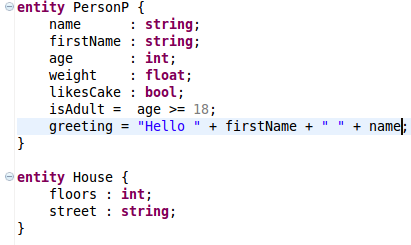
\includegraphics[width=\linewidth]{img/entities.png}

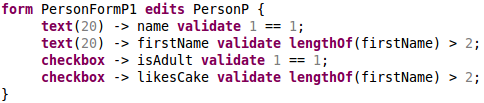
\includegraphics[width=\linewidth]{img/personform.png}

\end{frame}

\section{Plain Xtext}
\label{sec:plain-xtext}

To infer types, the plain Xtext scenario implements operations which determine
the actual type of an expression, the expected type (which depends on the
context where the expression is used), and operations which check whether a type
is assignable to another type (implemented in the classes
\mytt{GuiDslTypeProvider}, Section~\ref{sec:rectypecomputation}, and
\mytt{TypeConformance}, Section~\ref{sec:typeconformance}, respectively). The
Xtext validator, partially shown in listing \ref{lst:validation-plain}, uses
these operations.  The validation operating on text widgets checks that the type
of attribute the widget refers to is not \emph{boolean}.  The validation on
checkbox widgets, not shown in the listing, checks that the type is
\emph{boolean} in a similar way.
There is also a check which acts on any widget used to check whether the actual
type is assignable to the expected type, for instance \emph{boolean} for the
\emph{validate} clause of a widget. The expected type of an expression usually
depends on the context where the expression is in.
In case there is no expected type, for instance for an attribute whose type is
only defined by the derivation expression, the check operation just returns.
There is a similar check acting on any expression which basically makes sure
that the expression can be typed.

%class GuiDslTypeProvider {

	@Inject extension TypeConformance conformance
	
	// declare the built-in types for easy use
	Type bool = GuiDslFactory::eINSTANCE.createBooleanType
	Type _float = GuiDslFactory::eINSTANCE.createFloatType
	Type _int = GuiDslFactory::eINSTANCE.createIntType
	Type number = GuiDslFactory::eINSTANCE.createNumberType
	Type string = GuiDslFactory::eINSTANCE.createStringType
	Type primitive = GuiDslFactory::eINSTANCE.createPrimitiveType
	@Inject CyclicDependencyType cyclicType

	def Type getType(EObject e) {
		getType(e, newHashSet())
	}
	
	def Type getType(EObject e, Collection<EObject> visited) {
		if (visited.contains(e)) return cyclicType; // cycle detected
		visited.add(e)
		switch e {
			Widget : e.attr.getType(visited)
			Attribute case e.expr != null && e.type != null 
			   && e.type.isAssignable(e.expr.getType(visited)) : e.type
			Attribute case e.expr != null : e.expr.getType(visited)
			Attribute case e.type != null : e.type
			AttributeRef : e.attr.getType(visited)

			AndOrExpression : bool 
			Comparison : bool
			Equality : bool
			
			// type is the most general, e.g. int + float => float
			Plus : mostGeneral(e.left.getType(visited), e.right.getType(visited))
			Minus : mostGeneral(e.left.getType(visited), e.right.getType(visited))
			MultiOrDiv case e.op.equals("*"): mostGeneral(e.left.getType(visited),e.right.getType(visited))
			// as in Java
			MultiOrDiv case e.op.equals("/"): e.left.getType(visited)
			
			BooleanNegation : bool
			ArithmeticSigned : number
			
			// return type of attribute referenced by the widget
			FieldContent : return e.getContainerOfType(typeof(Widget))?.attr?.getType(visited)
			LengthOf : _int
			EntityType : e // type is itself
			BooleanLiteral : bool
			FloatLiteral : _float
			IntLiteral: _int
			StringLiteral : string

			default: null
		}
	} 
	def Type getExpectedType(EObject e) { 
		switch e {
			Widget : primitive
			default: internalGetExpectedType(e.eContainer, e.eContainingFeature) 
		}
	} 
	
	def protected Type internalGetExpectedType(EObject e, EStructuralFeature feature) {
		switch e {
			Widget case feature == GuiDslPackage$Literals::WIDGET__VALIDATE: bool
			
			Attribute case e.type != null : e.type
		
			AndOrExpression : bool 
			// an object contained (i.e. left or right side) 
			// in the following operator is expected to always be a number 
			Comparison : number
			// the left side of the operator determines the expected type 
			Equality : e.left.type
			// everything can be added, it might end up as string
			Plus :	mostGeneral(e.left.type, e.right.type).mostSpecific(string)
			Minus      : number
			MultiOrDiv : number

			BooleanNegation : bool
			ArithmeticSigned : number 
			
			LengthOf : string
			
			default : null
		}
	}
%linerange={15-23,31-42,49-57}
%\lstinputlisting[label=lst:validation-plain,caption=Xtext
% validator.,]{code/GuiDslJavaValidator.java}

\begin{lstlisting}[float=tb,label=lst:validation-plain,caption=Xtext validator.] 
public class GuiDslJavaValidator extends AbstractGuiDslJavaValidator {
	public final static String INCOMPATIBLE_TYPES = "incompatible_types";
	@Inject private GuiDslTypeProvider guiDslTypeProvider;
	@Inject private TypeConformance conformance;

	@Check
	public void check(TextWidget widget) {
		Type type = guiDslTypeProvider.getType(widget.getAttr());
		if (type.eClass() == GuiDslPackage.Literals.BOOLEAN_TYPE) {
			error("A text widget may not refer to a boolean attribute.",
					GuiDslPackage.Literals.WIDGET__ATTR, INCOMPATIBLE_TYPES);
		}
	}

	@Check
	void checkWidget(Widget widget) {
		checkType(widget, GuiDslPackage.Literals.WIDGET__ATTR);
	}
	
	@Check
	public void check(Expression expr) {
		checkType(expr, null);
	}
	
	protected void checkType(EObject object, EStructuralFeature feature) {
		Type expectedType = guiDslTypeProvider.getExpectedType(object);
		Type actualType = guiDslTypeProvider.getType(object);
		if (actualType instanceof CyclicDependencyType)
			error("Type is part of a cyclic dependency.", feature, INCOMPATIBLE_TYPES); return;
		if (expectedType == null) return;
		if (!conformance.isAssignable(expectedType, actualType)) {
			error("Incompatible types. Expected '" + expectedType
					+ "' but was '" + actualType + "'", feature,
					INCOMPATIBLE_TYPES);
		}
	}
}
\end{lstlisting}

\subsection{Recursive type computation}
\label{sec:rectypecomputation}

Listing \ref{lst:plain-type-provider1} shows parts of the recursive computation
of types, written in Xtend. The method \emph{getType()} determines the actual
type of an expression. It avoids endless loops in case of cyclic dependencies
(typically due to a malformed cyclic entity hierarchy) by caching already
calculated types.  The type of a primitive type model element as well as the
type of an entity is defined to be itself. The type of an attribute is its
declared type or the type of its initialization expression.
In case there are both an initialization expression and an explicit type, a
conformance check is made before (Section~\ref{sec:typeconformance}). If that
check fails, the default (\verb|null|) of the switch statement is returned.
References to attributes have the type of the referenced attribute, and the
\emph{widgetcontent} used in validate clauses has the type of the attribute that
the widget refers to.

%Note that \verb|e.type| is the reference to a (primitive) type while \verb|e.expr.type| and \verb|e.attr.type| recursively call \emph{getType()}. They use the Xtend 2 syntax shortcut to \verb|getType(e.expr.type)| and \verb|getType(e.attr.type)|. 

%\lstinputlisting[language=xtend,label=lst:plain-type-provider1,caption=Type
%provider in Xtend.]{code/GuiDslTypeProvider.xtend}

\begin{lstlisting}[language=xtend,float=tb,label=lst:plain-type-provider1,caption=Type provider in Xtend.] 
class GuiDslTypeProvider {
	@Inject extension TypeConformance conformance
	
	// declare the built-in types for easy use
	Type bool = GuiDslFactory::eINSTANCE.createBooleanType
	Type _float = GuiDslFactory::eINSTANCE.createFloatType
	// ... similar for other basic types
	@Inject CyclicDependencyType cyclicType

	def Type getType(EObject e) { getType(e, newHashSet()) }
	
	def Type getType(EObject e, Collection<EObject> visited) {
		if (visited.contains(e)) return cyclicType; // cycle detected
		visited.add(e)
		switch e {
			Widget : e.attr.getType(visited)
			Attribute case e.expr != null && e.type != null 
			   && e.type.isAssignable(e.expr.getType(visited)) : e.type
			Attribute case e.expr != null : e.expr.getType(visited)
			Attribute case e.type != null : e.type
			AttributeRef : e.attr.getType(visited)
			AndOrExpression : bool 
			Comparison : bool
			Equality : bool
			// type is the most general, e.g. int + float => float
			Plus : mostGeneral(e.left.getType(visited), e.right.getType(visited))
			Minus : mostGeneral(e.left.getType(visited), e.right.getType(visited))
			MultiOrDiv case e.op.equals("*"): mostGeneral(e.left.getType(visited),e.right.getType(visited))
			// as in Java
			MultiOrDiv case e.op.equals("/"): e.left.getType(visited)
			
			// similar for other expressions

			default: null
		}
	} 
	def Type getExpectedType(EObject e) {
		internalGetExpectedType(e.eContainer, e.eContainingFeature) 
	} 
}
\end{lstlisting}

The operation \emph{getExpectedType()} in listing \ref{lst:plain-type-provider1}
returns the expected type of an EObject by checking its container. It calls
another operation (not shown here) with the container of the EObject and the
feature of the container pointing to it. For instance, if the container of an
expression is a \emph{Widget} and the feature of the widget containing the
expression is the \emph{validate} clause, the expected type is boolean. If the
container is a \emph{Form} and the EObject a \emph{Widget}, the expected type
must be primitive (i.e., a widget cannot directly edit an entity).
The expected type of a subtraction, multiplication and division is a
\emph{NumberType}. For an addition, it is a string, unless there is a common
type of the summands that is more specific. The method returns \emph{null} to
indicate if there is no expected type.

%\lstinputlisting[label=lst:plain-type-provider2,caption=Calculating the expected type.,linerange={96-98,114-146}]{../org.typesys.guidsl/src/org/typesys/guidsl/types/GuiDslTypeProvider.xtend}

\subsection{Type conformance}
\label{sec:typeconformance}

An important part of type checking is whether another type can be provided where
a certain type is expected.
Listing \ref{lst:plain-type-conformance} shows the Xtend code to compute whether
a type is assignable to another, using polymorphic dispatch. The method
\emph{isAssignable(left, right)} returns true if an element of type \emph{right}
can be used where an element of type \emph{left} is expected.
Polymorphic dispatch is used, which means that a call to \emph{isAssignable()}
will be dispatched to the method with the most specific type parameters. The
most ``general'' method has the arguments \emph{(Type, Type)} and specifies that
a type can always be assigned to itself, or to one of its supertypes, using the
type hierarchy of the EMF model generated by the Xtext Grammar.
An entity can be assigned to another entity if it is of the same type (i.e., has
the same EMF \emph{EClass}), or if the latter is a super entity of the former.
Here, the reference \emph{superType} is not an EMF reference, but the one given
in the grammar for \emph{Entity}. Other special cases are dealt with the
following methods. As \emph{IntType} and \emph{FloatType} are on the same EMF
model inheritance hierarchy level, an assignment rule has to be explicitly
specified.

\begin{lstlisting}[language=xtend,float=tb,label=lst:plain-type-conformance,caption=Type
conformance specification (Xtend code).] 
class TypeConformance {
	def dispatch isAssignable(Type left, Type right) {
		left.eClass == right.eClass || right.eClass.EAllSuperTypes.contains(left.eClass) 
	}

	def dispatch isAssignable(EntityType left, EntityType right) {
		internalIsAssignable(left.ref, right.ref, newHashSet())
	}
	def internalIsAssignable(Entity left, Entity right, Collection<Entity> visited) {
		if (visited.contains(right)) return false; // cycle detected
		visited.add(right)
		left == right || (right.superType != null && 
			internalIsAssignable(left, right.superType, visited) )
	}
	
	def dispatch isAssignable(FloatType left, IntType right) { true }
	def dispatch isAssignable(StringType left, NumberType right) { true }

	def Type mostGeneral(Type one, Type two) {
		if (isAssignable(one, two)) one else two
	}
}
\end{lstlisting}

%\lstinputlisting[language=xtend,label=lst:plain-type-conformance,caption=Type
%conformance specification (Xtend code).]{code/TypeConformance.xtend}

% \subsection{Summary}
% The plain Xtext approach makes use of polymorphic dispatch and the Xtend syntax
% to keep the code concise, for instance with the Xtend \emph{switch} statement.
% It consists of four main parts:
% \begin{itemize}
% \item Xtend code to compute actual types recursively,
% \item an Xtend operation to compute expected types of expressions based on the container they are in,
% \item a type conformance specification, also written in Xtend, and
% \item the Xtext validator using all of the above.
% \end{itemize}


\def \xbaseImpl {Implementation in Xbase}
\section[Xbase]{\xbaseImpl}

\begin{frame}
  \frametitle{\xbaseImpl}
  \tableofcontents[currentsection]
\end{frame}
  
\begin{frame}[fragile]
  \frametitle{\xbaseImpl}
  \begin{itemize}
    \item Infer Java type for Entities and Forms with
    \emph{JvmModelInferrer}
  \end{itemize}
  \pause
  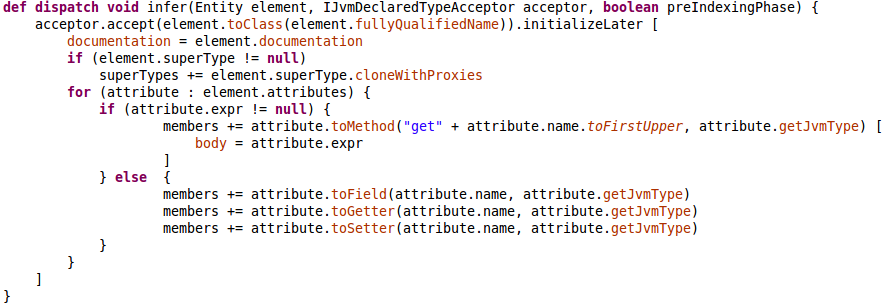
\includegraphics[width=1.1\textwidth]{img/xbase-infer.png}
  \pause
  \begin{itemize}
    \item Entity Attributes $\Rightarrow$ Xbase expressions, Java elements 
   \end{itemize}
  \note{Reuse JVM types by mapping to Java}
\end{frame}    

\note{
\begin{frame}
  \frametitle{\xbaseImpl}
  \begin{itemize}
    \item Entity Attributes $\Rightarrow$ Xbase expressions, Java elements 
   \end{itemize}
   \pause
  \begin{footnotesize}
  % Generator: GNU source-highlight, by Lorenzo Bettini, http://www.gnu.org/software/src-highlite
\begin{tabular}[t]{l}
\noindent
\mbox{}@Inject\ ITypeProvider\ typeProvider \\
\mbox{} \\
\mbox{}\textbf{\textcolor{Plum}{def}}\ JvmTypeReference\ \textcolor{Black}{getJvmType}(Attribute\ attr)\ \{ \\
\mbox{}\ \ \ \ \textbf{\textcolor{Plum}{switch}}\ attr\ \{ \\
\mbox{}\ \ \ \ \ \ \ \ Attribute\ \textbf{\textcolor{Plum}{case}}\ attr.type\ !=\ \textbf{\textcolor{Plum}{null}}\ :\ attr.type \\
\mbox{}\ \ \ \ \ \ \ \ Attribute\ \textbf{\textcolor{Plum}{case}}\ attr.expr\ !=\ \textbf{\textcolor{Plum}{null}}\ :\  \\
\mbox{}\ \ \ \ \ \ \ \ \ \ \ \ \ \ \ \ \ \ typeProvider.\textcolor{Black}{getType}(attr.\textcolor{Black}{getExpr}()) \\
\mbox{}\ \ \ \ \ \ \ \ \textbf{\textcolor{Plum}{default}}:\ \textbf{\textcolor{Plum}{null}} \\
\mbox{}\ \ \ \ \} \\
\mbox{}\}
\end{tabular}

  \end{footnotesize}
\end{frame}
}

\section{Xsemantics}
\label{sec:xsemantics}

Xsemantics~\cite{lbts} (the successor of Xtypes~\cite{Bet11}) is a DSL (written
in Xtext) for writing type systems, reduction rules, interpreters (and in
general relation rules) for languages implemented in Xtext.
A system definition in Xsemantics is a set of judgment rules which have a
conclusion and a set of premises; these rules can act on any Java object,
though, typically, they will act on EObjects which are elements of the metamodel
of the language implemented in Xtext.  Indeed, Xsemantics relies on Xbase to
provide a rich syntax for defining rules (and premises of rule), thus giving
full access to Java types.

Xsemantics is thought to be used by people who are at least a little familiar
with formal type systems and operational semantics: it aims at providing
a syntax which is close to the way deduction rules are written in a formal
setting~\cite{hindley:1997a,Pierce02}.
Actually, Xsemantics rules are written in the other direction with respect
to standard deduction rules: the conclusion come before the premises; this is just
to make IDE tooling work better, and to give a more "programming" style to rules.

Starting from the definitions of these rules, Xsemantics generates Java code
that can be used in your language implemented in Xtext for scoping and
validation (it also generates a validator in Java).  Xsemantics aims at
providing a rich syntax for defining any kind of rules: relations among elements
(e.g., \emph{subtyping}), \emph{static semantics} (i.e., type systems) and
\emph{dynamic semantics} (i.e., reduction rules that can be used for
interpreting a program).  In this paper, we will use it for writing the rules of
the type system of the case study we are considering
(Section~\ref{sec:casestudy}).

\subsection{Type System Specification}

The first thing to do in a system defined in Xsemantics, after giving it a name,
is to declare the \emph{judgments} of your system; a judgment consists of

\begin{itemize}
\item 
a name, which has to be unique in the system;
\item 
a \textit{judgment symbol} that can be chosen from some predefined symbols;
\item 
the \textit{parameters} of the judgment; parameters of a judgments are separated by
	a \textit{relation symbol} that can be chosen from some predefined symbols;
\end{itemize}

\noindent
The parameters can be

\begin{itemize}
\item 
input parameters, in that case they are declared as Java parameters;
\item 
output parameters, in that case you use the keyword
\verb|output| followed by the Java
type of the output parameter.
\end{itemize}

\begin{lstlisting}[language=xsemantics,float,label=lst:xsemantics-judgments,caption=Judgment
definitions in Xsemantics]
system org.typesys.xsem.guidsl.xsemantics.TypeSystem

import org.typesys.xsem.guidsl.xsemGuiDsl.*

judgments {
	attrtype ||- Attribute attribute : output Type
	exprtype |- Expression expression : output Type
	// whether {@code right} is assignable to {@code left}
	isAssignable |- Type left <~ Type right
	// computes the most general type between {@code first} and {@code second}
	mostGeneral |- Type first ~~  Type second |> output Type
}
\end{lstlisting}

\noindent
The judgment definitions for our case study are shown in
Listing~\ref{lst:xsemantics-judgments}.

Once the judgments of the system are declared, we can start declaring the
rules.  Each rule consists of

\begin{itemize}
\item
a name, which has to be unique in the system;
\item
a \textit{rule conclusion};
\item
the \textit{premises} of the rule;
\end{itemize}

\noindent
The rule conclusion consists of

\begin{itemize}
\item
the name of the \textit{environment} of a rule;
\item
a \textit{judgment symbol};
\item
the \textit{parameters} of the rules, which are separated by
a \textit{relation symbol} that can be chosen from some predefined symbols;
\end{itemize}

The things that make a rule belong to a specific judgment are the judgment
symbol, the relation symbols (which separate the parameters); moreover the types
of the parameters of a rule must be (Java) subtypes of the corresponding types
of the judgment (or exactly the same Java types).  Two rules belonging to the
same judgment must differ for at least one input parameter's type.

The premises of a rule which are specified in a \verb|from| block can be any
Xbase expression, or a rule invocation.  If you think of a rule declaration as a
function declaration, then a rule invocation corresponds to function invocation,
thus you must specify the environment to pass to the rule, and the arguments,
both input and output arguments.
Moreover, if a rule does not require any premise, we can use a special form of
rules, called indeed \textit{axiom}s, which only have a conclusion, without
premises.

At runtime, the system will select the most appropriate rule according
to the runtime types of the passed argument (similar to
\textit{polymorphic dispatch} mechanism).

In the premises you can assign values to the output parameters; and
when you invoke another rule, upon return, the output arguments will have
the values assigned in the invoked rule.

If one of the premises fails, then the whole rule will fail, and in turn all the
stack of rule invocation will fail.  If the premise is a boolean expression, it
will fail if the expression evaluates to false.  If the premise is a rule
invocation, it will fail if the invoked rule fails.

\begin{lstlisting}[language=xsemantics]
axiom SimpleAttributeType
	G ||- SimpleAttribute attr : attr.type

rule DerivedAttributeType
	G ||- DerivedAttribute attr : Type attrType
from {
	G |- attr.expr : attrType
}
\end{lstlisting}

\subsection{Usage in Xtext}

With the declarative specification (written in the Xsemantics DSL), Java methods are generated that can be used in the SopeProvider or Validators. 

If the declarative rules are marked with […], Xtext validator classes are directly created and no further work is necessary.

Example output for reusable methods

\begin{lstlisting}
TypeSystemResult<MyOtherGrammarElement> typeAsMyOtherGrammarElement(MyGrammarElement left); 
TypeSystemResult<MyGrammarElement, MyOtherGrammarElement> type(MyGrammarElement left, MyOtherGrammarElement right); 
TypeSystemResult<Boolean> checkType(MyGrammarElement left, MyOtherGrammarElement right); 
\end{lstlisting}

\section[XTS]{Implementation in XTS}

\begin{frame}
  \frametitle{Xtext Typesystem (XTS)}
  \tableofcontents[currentsection]
\end{frame}

\begin{frame}
  \frametitle{Xtext Typesystem (XTS)}
  \begin{itemize}
  \item Typesystem DSL written in Xtext
  \item Additional uses: interpreter, testing
  \item Recursive type computation
\end{itemize}
\end{frame}

\begin{frame}[fragile]
  \frametitle{The Plus Operator with XTS}

  \begin{itemize}
    \item Commonly used language elements 
  \end{itemize}

  \begin{footnotesize}
    % Generator: GNU source-highlight, by Lorenzo Bettini, http://www.gnu.org/software/src-highlite
\begin{tabular}[t]{l}
\noindent
\mbox{}\textbf{\textcolor{Plum}{subtype}}\ FloatType\ \textbf{\textcolor{Plum}{base}}\ IntType \\
\mbox{} \\
\mbox{}\textbf{\textcolor{Plum}{characteristic}}\ NUMERIC\ \{ \\
\mbox{}\ \ \ \ IntType,\ FloatType \\
\mbox{}\}\  \\
\mbox{} \\
\mbox{}\textbf{\textcolor{Plum}{typeof}}\ Plus\ -$>$\ \textbf{\textcolor{Plum}{common}}\ left\ right\ \{ \\
\mbox{}\ \ \ \ \textbf{\textcolor{Plum}{ensureType}}\ left\ :$<$=:\ StringType,\ \textbf{\textcolor{Plum}{char}}(NUMERIC) \\
\mbox{}\ \ \ \ \textbf{\textcolor{Plum}{ensureType}}\ right\ :$<$=:\ StringType,\ \textbf{\textcolor{Plum}{char}}(NUMERIC) \\
\mbox{}\ \ \ \ \textbf{\textcolor{Plum}{ensureCompatibility}}\ left\ :$<$=$>$:\ right \\
\mbox{}\} \\
\mbox{}
\end{tabular}

  \end{footnotesize}

  \note{
  \begin{itemize}
    \item subtype relationships
    \item grouping of types
    \item type computation, \emph{ensure}\ldots clauses 
  \end{itemize}}
  
\note{
\begin{frame}[fragile]
  \frametitle{The Plus Operator with XTS}
  \begin{itemize}
    \item Coercion of a number to a String
  \end{itemize}

  \begin{footnotesize}
    % Generator: GNU source-highlight, by Lorenzo Bettini, http://www.gnu.org/software/src-highlite
\begin{tabular}[t]{l}
\noindent
\mbox{}\textbf{\textcolor{Plum}{public}}\ EObject\ \textcolor{Black}{typeCoerce}(\ EObject\ candidateElement,\ FloatType\ candidate,\  \\
\mbox{}\ \ \ \ \ \ \ \ StringType\ expected,\ TypeCalculationTrace\ trace\ )\ \{ \\
\mbox{}\ \ \ \ \textbf{\textcolor{Plum}{if}}\ (\ candidateElement\ \textbf{\textcolor{Plum}{instanceof}}\ NumberLiteral\ )\ \{ \\
\mbox{}\ \ \ \ \ \ \ \ \ \ \ \ trace.\textcolor{Black}{add}(\ candidateElement,\ \textcolor{RoyalBlue}{"{}Number\ coerced\ to\ string."{}}); \\
\mbox{}\ \ \ \ \ \ \ \ \ \ \ \ \textbf{\textcolor{Plum}{return}}\ \textcolor{Black}{create}(cl.\textcolor{Black}{getStringType}()); \\
\mbox{}\ \ \ \ \} \\
\mbox{}\ \ \ \ \textbf{\textcolor{Plum}{return}}\ \textbf{\textcolor{Plum}{null}}; \\
\mbox{}\}
\end{tabular}

  \end{footnotesize}

  \begin{itemize}
    \item XTS will try custom coercion methods before throwing a type error
    \item coercion methods use polymorphic dispatch 
  \end{itemize}
  public EObject typeCoerce( EObject candidateElement, FloatType candidate, 
		StringType expected, TypeCalculationTrace trace ) {
	if ( candidateElement instanceof NumberLiteral ) {
			trace.add( candidateElement, "Number coerced to string.");
			return create(lang.getStringType());
	}
	return null;
}
\end{frame}}	
\end{frame}

\section{Comparison}

\begin{frame}[fragile,allowframebreaks]
  \frametitle{Which approach to use when?}
  
  Criteria to help in deciding which approach might be good for a particular use
  case:
  \begin{itemize}
    \item Context: coupling of the DSL with Java
    \item Expressivity
    \item Verbosity/conciseness
    \item Customizability
    \item Additional features
    \item Target audience
    \item Learning curve
    \item Documentation
    \item Support
  \end{itemize}

\framebreak  
\begin{tabularx}{\linewidth}{ l   X }
\multicolumn{2}{c}{Context: coupling of the DSL with Java} \\ \hline
Plain & DSL may refer to \emph{JavaVMTypes} as known from Xtext 1\\
Xbase & Tight coupling, DSL may link to Java classes, \emph{JvmModelInferrer}
generates Java classes from DSL model elements\\
Xsem & see \emph{Plain} \\
XTS & see \emph{Plain} \\
\end{tabularx}
\begin{itemize}
  \item \emph{JavaVMTypes}: use \emph{import
  ``http://\-www.eclipse.org/\-xtext/\-common/\-JavaVMTypes'' \ldots}
  \item All approaches allow to hook in custom java methods for typing rule
  computation
\end{itemize}

\framebreak
\begin{tabularx}{\linewidth}{ l   X }
\multicolumn{2}{c}{Expressivity} \\ \hline
Plain & Java \\
Xbase & Xbase library \\
Xsem & similar to Xbase + specific syntax\\
XTS & EMF feature access + specific syntax\\
\end{tabularx}

\framebreak
\begin{tabularx}{\linewidth}{ l   X }
\multicolumn{2}{c}{Verbosity/conciseness} \\ \hline
Plain & Xtend, \emph{TypeProvider}, \emph{TypeConformance}, $\approx$300 LOC\\
Xbase & Xtend, \emph{JvmModelInferrer}, reuse Java types, $\approx$200 LOC  \\
Xsem &  -, $\approx$200 LOC \\
XTS & -, $\approx$70 LOC\\
\end{tabularx}

TODO: Numbers are just placeholders, define what goes into LOC and then count,
count characters instead of LOC?

\framebreak
\begin{tabularx}{\linewidth}{ l   X }
\multicolumn{2}{c}{Customizability} \\ \hline
Plain & no framework, change source \\
Xbase & Xbase and Xtext framework \\
Xsem & write custom Java methods (generation GAP
pattern)
\\
XTS & hooks for own implementations \\
\end{tabularx}

\framebreak
\begin{tabularx}{\linewidth}{ l   X }
\multicolumn{2}{c}{Additional Features} \\ \hline
Plain & - \\
Xbase & generated Java classes for free \\
Xsem & dynamic type checking and interpreters, generates validators \\
XTS & \ldots, generates validators \\
\end{tabularx}

\framebreak
\begin{tabularx}{\linewidth}{ l   X }
\multicolumn{2}{c}{Target audience} \\ \hline
Plain & - \\
Xbase & - \\
Xsem & people familiar with formal systems \\
XTS & - \\
\end{tabularx}

\framebreak
\begin{tabularx}{\linewidth}{ l   X }
\multicolumn{2}{c}{Learning curve} \\ \hline
Plain & Xtend \\
Xbase & Xbase, JVM Model inferrer from Xtext Documentation \\
Xsem & similar to rules written in commonly used type theory \\
XTS & - \\
\end{tabularx}

\framebreak
\begin{tabularx}{\linewidth}{ l   X }
\multicolumn{2}{c}{Documentation} \\ \hline
Plain & Xtext/Xtend in general \\
Xbase & Xtext documentation JvmModelInferrer \\
Xsem & http://xsemantics.sourceforge.net/ \\
XTS & http://code.google.com/a/eclipselabs.org/p/xtext-typesystem/ \\
\end{tabularx}

\framebreak
\begin{tabularx}{\linewidth}{ l   X }
\multicolumn{2}{c}{Support} \\ \hline
Plain & - \\
Xbase & - \\
Xsem & - \\
XTS & - \\
\end{tabularx}
  
\end{frame}
\section{Conclusion and Related Work}
\label{sec:conclusion}

\newcommand{\xtypes}{XTypeS}
\newcommand{\xtext}{Xtext}

A typical way of declaring constraints in metamodels is to use OCL (Object
Constraint Language) \cite{WarmerKleppe99,OCLOMG}.  OCL is an expression
language, while our \xtypes{} is based on type system rules; furthermore, while
OCL is suitable for specifying constraints, it might be hard to use to perform
type inference.

There are other tools for implementing DSLs and their text editors with IDE
functionalities (we also refer to \cite{PP08} for a comparison). Tools like IMP
(The IDE Meta-Tooling Platform) \cite{imp09} and DLTK (Dynamic Languages
Toolkit) \cite{DLTK} only deal with IDE functionalities. TCS (Textual Concrete
Syntax) \cite{tcs} is similar to \xtext, but with the latter it is easier to
describe the abstract and concrete syntax at once, and it is completely open to
customization of every part of the generated IDE (besides, TCS seems to be no
longer under active development). EMFText~\cite{emftext09}, instead of deriving
a metamodel from the grammar, does the opposite, i.e., the language to be
implemented must be defined in an abstract way using an EMF metamodel. Since
also EMFText relies on EMF we believe that \xtypes{} could also be used with
this tool, though we still have not investigated this issue.
Spoofax~\cite{Spoofax2010}, another language workbench which targets Eclipse,
fosters agile language design and development (e.g., changes to the language can
be dynamically loaded into the environment); it does not require Java code for
the analysis of a program (and other IDE related mechanisms) since it relies on
Stratego~\cite{Stratego2008} for rule-based specifications.  With this respect,
\xtypes{} tries to fill the gap concerning the typing of programs, which in
\xtext{} which still requires Java programming, with a type system DSL.

EriLex~\cite{EriLex} is a software tool for generating support code for embedded
domain specific languages and it supports specifying syntax, type rules, and
dynamic semantics of such languages but it does not generate any artifact for
IDE functionalities. MPS (Meta Programming System) \cite{MPS} is another tool
for developing a DSL, and it also provides IDE functionalities, but it does not
target Eclipse and its well-known functionalities.

There are older works that aim at providing complete frameworks for language
implementation (both compilation and editing environment), such as
\emph{Synthesizer}~\cite{Synthesizer} and \emph{Centaur}~\cite{Centaur} (the
former relying on its own specification language and the latter relying on Lisp,
Prolog and other formalisms \cite{Metal,PPML,Typol}). \xtext{} shares with
these tools the philosophy that the editing part is crucial for the programming
(in particular the immediate feedback about problems in the program being
editing~\cite{Synthesizer}) and thus a framework for implementing languages
should address also this functionality.  \xtext, and then \xtypes, aim at
providing these functionalities on top of the widely used Eclipse platform and
by relying on EMF which is a very useful framework for modeling and manipulation
of models (in this case the AST of the programs).

Although \xtypes{} was designed and developed to be used in a language
implemented in \xtext, rules written in \xtypes{} do not refer to the syntax of
the language elements, but only to the structure of the model representing the
AST.  Differently from other approaches, such as, e.g.,
\cite{Centaur,MPS,ASFSDF,Ruler,PLTRedex,EriLex,Neverlang2010}, which require the
programmer to use the framework also for defining the syntax of the language, a
type system written in \xtypes{} only needs an EMF metamodel, i.e., the
\emph{ecore} file (in our context, it is the one generated by \xtext). Thus, the
Java code generated by \xtypes{} might also be used to validate any EMF model,
independently from \xtext{} itself.  Indeed, it might be used with any other
frameworks that represent a program in the shape of an EMF model (though in that
case, Java code generation might have to be adapted).

Neverlang \cite{Neverlang2010} is based on the fact that programming language
features can be easily plugged and unplugged. Similarly, \cite{JastAdd} supports
modular specifications of extensible compiler tools and languages.
Spoofax~\cite{Spoofax2010} provides support for language extensions and
embeddings. \xtext{} provides mechanisms for reusing and composing grammars (we
refer to \xtext{} documentation~\cite{xtext}), but at the moment these
mechanisms may require some manual programming w.r.t.\ the automatic
mechanisms of the above mentioned works. However, from the type system point of
view, since \xtypes{} is only connected to the EMF metamodel (and not to the
grammar), we think that it can be used for modular implementation of type system
related functionalities and in particular for implementing \emph{pluggable type
systems}~\cite{Brac04a}.

\xtypes{} does not aim at providing mechanisms for formal proofs for the
language and the type system; for instance, it does not produce, like other
frameworks do (see, e.g., \cite{Ott}), versions of the type system for proof
assistants like Coq~\cite{Coq}, HOL~\cite{HOL} or Isabelle~\cite{Isabelle}.
Although this issue still needs further investigation, we think that
specifications of rules in \xtypes{} might be good candidates for such generated
definitions for proof assistants.

Finally, we just mention here other tools and frameworks for implementation of
DSLs that are different from \xtext{} and \xtypes{} basically for the main goal
and programming context, such as, e.g., \cite{JST98,MetaBorg06,MontiCore10}
which are based on language specification preprocessors,
\cite{XMF08,LanguageBoxes09} which target host language extensions and internal
DSLs, \cite{ASFSDF,Ruler,PLTRedex} which do not target IDE functionalities. We
would also like to stress that, since \xtypes{} is implemented in \xtext{}
itself, it also provides a full feature Eclipse-based editor for writing the
type system with all the standard IDE functionalities, which is something that
the mentioned related works do not provide.


\appendix
\section[Appendix]{Appendix}

% The following slides are not shown in the table of contents 

\begin{frame}
  \frametitle{Appendix}
\end{frame}

\end{document}


%%% Local Variables:
%%% mode: latex
%%% TeX-master: "presentation"
%%% End: